% !TEX options=--shell-escape
\documentclass [12pt]{article} 

\usepackage {amsmath}
\usepackage {amsthm}
\usepackage {amssymb}
\usepackage {graphicx} 
\usepackage {float}
\usepackage {multirow}
\usepackage {xcolor}
\usepackage {algorithmic}
\usepackage [ruled,vlined,commentsnumbered,titlenotnumbered]{algorithm2e} \usepackage {array} 
\usepackage {booktabs} 
\usepackage {url} 
\usepackage {parskip} 
\usepackage [margin=1in]{geometry} 
\usepackage [T1]{fontenc} 
\usepackage {cmbright} 
\usepackage [many]{tcolorbox} 
\usepackage [colorlinks = true,
            linkcolor = blue,
            urlcolor  = blue,
            citecolor = blue,
            anchorcolor = blue]{hyperref} 
\usepackage {enumitem} 
\usepackage {xparse} 
\usepackage {verbatim}
\usepackage{listings}
\usepackage{xcolor}
\usepackage{csquotes}
\usepackage[cache=false]{minted}
\usepackage{mdframed}
\usepackage{tikz}
\usetikzlibrary{shapes.symbols}
\newtheorem{theorem}{Theorem}

\BeforeBeginEnvironment{minted}{\begin{mdframed}}
\AfterEndEnvironment{minted}{\end{mdframed}}

\DeclareTColorBox {Solution}{}{breakable, title={Solution}}
\DeclareTColorBox {Solution*}{}{breakable, title={Solution (provided)}}
\DeclareTColorBox {Instruction}{}{boxrule=0pt, boxsep=0pt, left=0.5em, right=0.5em, top=0.5em, bottom=0.5em, arc=0pt, toprule=1pt, bottomrule=1pt}
\DeclareDocumentCommand {\Expecting }{+m}{\textbf {[We are expecting:} #1\textbf {]}}
\DeclareDocumentCommand {\Points }{m}{\textbf {(#1 pt.)}} 
\newcommand {\hint }[1]{\noindent {[\textbf {HINT:} \em #1 \em ]}} \newcommand {\pts }[1]{\textbf {(#1 pt.)}} 

\begin{document} 

{\LARGE \textbf {COMP 285 (NC A\&T, Spr `22)}\hfill \textbf {Homework 6} } 
\vspace {1em} 
\begin{Instruction} 

\paragraph {Due.} Wednesday, March 23rd, 2022 @ 11:59 PM!
\end{Instruction} 

\vspace {1em} 
\begin{Instruction} \paragraph {Homework Expectations:} Please see \href{https://www.comp285.ml/homework/#general-homework-information}{Homework}.
\end{Instruction}

\vspace {1em} 
\begin{Instruction} 

\paragraph {Exercises} The following questions are exercises. We encourage you to work with a group and discuss solutions to make sure you understand the material.

\paragraph {Points} This assignment is graded out of 100 points. However, you can get up to 120 points if you complete everything. These are not bonus points, but rather points to help make-up any parts you miss.

\end{Instruction} 

\begin{centering}
\section*{Fun with Graphs}
\end{centering}

\begin{Instruction}

\paragraph{Written Problems} The following questions are to be submitted in written/typed form to gradescope.

\end{Instruction}

\section{Exercise: DFS Basics \Points{12}}
\label{sec:last}

Consider the following directed acyclic graph (DAG): 

\begin{center}
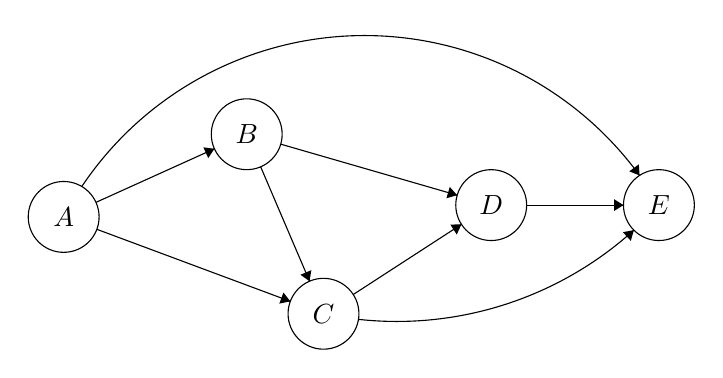
\begin{tikzpicture}[scale=0.15] 
    \tikzstyle{every node}+=[inner sep=0pt]
    \draw [black] (18.2,-24.6) circle (3);
    \draw (18.2,-24.6) node {$A$}; 
    \draw [black] (33.7,-17.6) circle (3);
    \draw (33.7,-17.6) node {$B$};
    \draw [black] (40.2,-32.8) circle (3);
    \draw (40.2,-32.8) node {$C$};
    \draw [black] (54.4,-23.6) circle (3);
    \draw (54.4,-23.6) node {$D$};
    \draw [black] (68.6,-23.6) circle (3);
    \draw (68.6,-23.6) node {$E$};
    \draw [black] (57.4,-23.6) -- (65.6,-23.6);
    \fill [black] (65.6,-23.6) -- (64.8,-23.1) -- (64.8,-24.1);
    \draw [black] (20.93,-23.37) -- (30.97,-18.83);
    \fill [black] (30.97,-18.83) -- (30.03,-18.71) -- (30.44,-19.62);
    \draw [black] (34.88,-20.36) -- (39.02,-30.04);
    \fill [black] (39.02,-30.04) -- (39.17,-29.11) -- (38.25,-29.5);
    \draw [black] (42.72,-31.17) -- (51.88,-25.23);
    \fill [black] (51.88,-25.23) -- (50.94,-25.25) -- (51.48,-26.09);
    \draw [black] (21.01,-25.65) -- (37.39,-31.75);
    \fill [black] (37.39,-31.75) -- (36.81,-31) -- (36.46,-31.94);
    \draw [black] (36.58,-18.44) -- (51.52,-22.76);
    \fill [black] (51.52,-22.76) -- (50.89,-22.06) -- (50.61,-23.02);
    \draw [black] (19.736,-22.025) arc (146.19641:36.07693:28.811);
    \fill [black] (66.96,-21.09) -- (66.9,-20.15) -- (66.09,-20.74);
    \draw [black] (66.48,-25.721) arc (-47.8655:-96.2357:29.916);
    \fill [black] (66.48,-25.72) -- (65.55,-25.89) -- (66.22,-26.63);
\end{tikzpicture} 
\end{center} 

In class, we saw how to use DFS to find a topological ordering of the the vertices; in the graph above, the unique topological ordering is $A,B,C,D,E$. We saw an example where we happened to start DFS from the first vertex in the topological order. In this exercise we'll see what happens when we start at a different vertex. Recall that when you run DFS, if it reached a node with no children (i.e. can't go any further), then it will resume the search at an unvisited vertex. 


\subsection {\Points {6}} 

Run DFS starting at vertex $C$, breaking any ties by alphabetical order.\footnote {For example, if DFS has a choice between $B$ or $C$, it will always choose $B$. This includes when DFS is starting a new tree in the DFS forest.}

\begin{enumerate}[label=(\alph *)]
    \item \Points{3} What do you get when you order the vertices by \textbf {ascending} start time?
    \item \Points{3} What do you get when you order the vertices by \textbf {descending} finish time?
\end{enumerate} 

\subsection {\Points {6}}

Run DFS starting at vertex $C$, breaking any ties by \textbf {reverse} alphabetical order.\footnote {For example, when DFS has a choice between $B$ or $C$, it will always choose $C$. This includes when DFS is starting a new tree in the DFS forest.}

\begin{enumerate}[label=(\alph *)]
    \item \Points{3} What do you get when you order the vertices by \textbf {ascending} start time?
    \item \Points{3} What do you get when you order the vertices by \textbf {descending} finish time?
\end{enumerate} 

\Expecting {For all four questions, an ordering of vertices. No justification is required.} 


\pagebreak
\section{Exercise: The World as Graphs \Points{12}}
For each of the following real-world problems, try to formulate this as a problem about graphs.

Recall a graph is just a collection of vertices and edges.

What algorithmic problem about graphs do we need to solve in order to solve the following
problems? (Note, you don't actually have to solve these problems, just transform them into
graph problems that we might then be able to solve).

\begin{enumerate}
    \item \Points{4} Among actors, a ``Bacon number'' is the number of degrees of separation from an actor to Kevin Bacon. For example, Kevin Bacon's Bacon number is $0$. If an actor works in a movie with Kevin Bacon, the actor's Bacon number is $1$. If an actor $A$ works with an actor $B$ who worked with Kevin Bacon in a movie, then actor $A$'s Bacon number is $2$, and so forth. How would you represent this as a graph so we could answer questions like: (a) What is Samuel L. Jackson's Bacon number? and (b) list all the people with Bacon number equal to 6.

    \item \Points{4} You need to take a bunch of classes at North Carolina A\&T University, and some of them depend on each other. For example, you must take COMP 280 before taking COMP 285.Given a set of classes you need to take, and information about which class is a pre-requisite for which other class, generate an order in which to take all of the classes. Assume you can only take one class at a time. How would you repesent this as a graph so we can answer this question?

    \item \Points{4} You are about to purchase a bunch of fish. You have two very large fishtanks. Unfortunately, some of these species of fish will fight if they are put in the same tank. For each pair of species, you know whether they will fight or whether they will peacefully co-exist. How would you represent this as a graph such that you can find a way to separate the fish into two peaceful fishtanks if it exists.
\end{enumerate}

\Expecting{For each of the three questions above, explain how you'd represent them as graphs. What are the nodes? What are the edges? Are the edges directed? Are they weighted?}

\pagebreak
\section{Exercise: Kosaraju’s algorithm \Points{16}}
\begin{center}
    \tikzset{every picture/.style={line width=0.75pt}} %set default line width to 0.75pt        

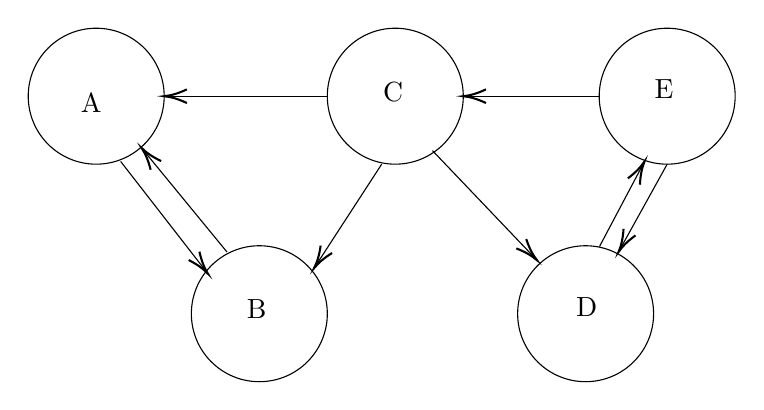
\begin{tikzpicture}[x=0.75pt,y=0.75pt,yscale=-1,xscale=1]
%uncomment if require: \path (0,300); %set diagram left start at 0, and has height of 300

%Shape: Ellipse [id:dp9466726400354856] 
\draw   (12,42.75) .. controls (12,24.66) and (26.66,10) .. (44.75,10) .. controls (62.84,10) and (77.5,24.66) .. (77.5,42.75) .. controls (77.5,60.84) and (62.84,75.5) .. (44.75,75.5) .. controls (26.66,75.5) and (12,60.84) .. (12,42.75) -- cycle ;
%Shape: Ellipse [id:dp8488568374172225] 
\draw   (90.6,147.55) .. controls (90.6,129.46) and (105.26,114.8) .. (123.35,114.8) .. controls (141.44,114.8) and (156.1,129.46) .. (156.1,147.55) .. controls (156.1,165.64) and (141.44,180.3) .. (123.35,180.3) .. controls (105.26,180.3) and (90.6,165.64) .. (90.6,147.55) -- cycle ;
%Shape: Ellipse [id:dp155526197737751] 
\draw   (156.1,42.75) .. controls (156.1,24.66) and (170.76,10) .. (188.85,10) .. controls (206.94,10) and (221.6,24.66) .. (221.6,42.75) .. controls (221.6,60.84) and (206.94,75.5) .. (188.85,75.5) .. controls (170.76,75.5) and (156.1,60.84) .. (156.1,42.75) -- cycle ;
%Shape: Ellipse [id:dp3865239171217767] 
\draw   (287.1,42.75) .. controls (287.1,24.66) and (301.76,10) .. (319.85,10) .. controls (337.94,10) and (352.6,24.66) .. (352.6,42.75) .. controls (352.6,60.84) and (337.94,75.5) .. (319.85,75.5) .. controls (301.76,75.5) and (287.1,60.84) .. (287.1,42.75) -- cycle ;
%Shape: Circle [id:dp6765767240776946] 
\draw   (247.8,147.55) .. controls (247.8,129.46) and (262.46,114.8) .. (280.55,114.8) .. controls (298.64,114.8) and (313.3,129.46) .. (313.3,147.55) .. controls (313.3,165.64) and (298.64,180.3) .. (280.55,180.3) .. controls (262.46,180.3) and (247.8,165.64) .. (247.8,147.55) -- cycle ;
%Straight Lines [id:da30984708629827207] 
\draw    (56.54,74.19) -- (97.36,126.71) ;
\draw [shift={(98.59,128.29)}, rotate = 232.14] [color={rgb, 255:red, 0; green, 0; blue, 0 }  ][line width=0.75]    (10.93,-3.29) .. controls (6.95,-1.4) and (3.31,-0.3) .. (0,0) .. controls (3.31,0.3) and (6.95,1.4) .. (10.93,3.29)   ;
%Straight Lines [id:da8022996189505263] 
\draw    (107.76,117.81) -- (67.85,69.19) ;
\draw [shift={(66.58,67.64)}, rotate = 50.62] [color={rgb, 255:red, 0; green, 0; blue, 0 }  ][line width=0.75]    (10.93,-3.29) .. controls (6.95,-1.4) and (3.31,-0.3) .. (0,0) .. controls (3.31,0.3) and (6.95,1.4) .. (10.93,3.29)   ;
%Straight Lines [id:da4961222933159456] 
\draw    (156.1,42.75) -- (79.5,42.75) ;
\draw [shift={(77.5,42.75)}, rotate = 360] [color={rgb, 255:red, 0; green, 0; blue, 0 }  ][line width=0.75]    (10.93,-3.29) .. controls (6.95,-1.4) and (3.31,-0.3) .. (0,0) .. controls (3.31,0.3) and (6.95,1.4) .. (10.93,3.29)   ;
%Straight Lines [id:da5592537989858153] 
\draw    (182.3,75.5) -- (150.77,124) ;
\draw [shift={(149.68,125.67)}, rotate = 303.03] [color={rgb, 255:red, 0; green, 0; blue, 0 }  ][line width=0.75]    (10.93,-3.29) .. controls (6.95,-1.4) and (3.31,-0.3) .. (0,0) .. controls (3.31,0.3) and (6.95,1.4) .. (10.93,3.29)   ;
%Straight Lines [id:da4738419319263515] 
\draw    (206.75,68.95) -- (255.72,120.3) ;
\draw [shift={(257.1,121.74)}, rotate = 226.36] [color={rgb, 255:red, 0; green, 0; blue, 0 }  ][line width=0.75]    (10.93,-3.29) .. controls (6.95,-1.4) and (3.31,-0.3) .. (0,0) .. controls (3.31,0.3) and (6.95,1.4) .. (10.93,3.29)   ;
%Straight Lines [id:da7891493345502749] 
\draw    (287.23,115.19) -- (308,75.96) ;
\draw [shift={(308.93,74.19)}, rotate = 117.89] [color={rgb, 255:red, 0; green, 0; blue, 0 }  ][line width=0.75]    (10.93,-3.29) .. controls (6.95,-1.4) and (3.31,-0.3) .. (0,0) .. controls (3.31,0.3) and (6.95,1.4) .. (10.93,3.29)   ;
%Straight Lines [id:da3951948209924262] 
\draw    (287.1,42.75) -- (223.6,42.75) ;
\draw [shift={(221.6,42.75)}, rotate = 360] [color={rgb, 255:red, 0; green, 0; blue, 0 }  ][line width=0.75]    (10.93,-3.29) .. controls (6.95,-1.4) and (3.31,-0.3) .. (0,0) .. controls (3.31,0.3) and (6.95,1.4) .. (10.93,3.29)   ;
%Straight Lines [id:da9073416168418074] 
\draw    (319.85,75.5) -- (297.37,116.06) ;
\draw [shift={(296.4,117.81)}, rotate = 298.99] [color={rgb, 255:red, 0; green, 0; blue, 0 }  ][line width=0.75]    (10.93,-3.29) .. controls (6.95,-1.4) and (3.31,-0.3) .. (0,0) .. controls (3.31,0.3) and (6.95,1.4) .. (10.93,3.29)   ;

% Text Node
\draw (36.13,40.15) node [anchor=north west][inner sep=0.75pt]   [align=left] {A};
% Text Node
\draw (116.04,139.71) node [anchor=north west][inner sep=0.75pt]   [align=left] {B};
% Text Node
\draw (181.7,34.91) node [anchor=north west][inner sep=0.75pt]   [align=left] {C};
% Text Node
\draw (274.71,138.4) node [anchor=north west][inner sep=0.75pt]   [align=left] {D};
% Text Node
\draw (312.54,33.6) node [anchor=north west][inner sep=0.75pt]   [align=left] {E};


\end{tikzpicture}
\end{center}

In this question, we ask you to run Kosarju's SCC algorithm (see Lecture 18, Slide 45). We summarize the gist here:

When running DFS, we will \textbf{break any ties by alphabetical order}. Remember that if DFS has reached a node with no un-visited children (i.e. can’t go any further), then it will resume the search at an unvisited vertex. We will decide which unexplored vertex to continue DFS by \textbf{alphabetical order}.


\subsection{First DFS \Points {4}}
What are the start and finish times of each node after running the first DFS from node $C$ on the \textbf {original} graph?

\begin{tabular}{c| c| c}
Node & Start Time & Finish Time \\ 
\hline A & & \\ 
\hline B & & \\ 
\hline C & 0 & \\ 
\hline D & & \\ 
\hline E & & \\ 
\end{tabular} 

\Expecting {Fill in this table}  

\subsection{Second DFS \Points {6}} 

Next, we will run DFS from the node with the largest finish time on the \textbf{reversed} graph. What do you get when you order the vertices by \textbf{ascending} start time for the second DFS run? 

\Expecting{An ordering of vertices. No justification is required}  

\subsection{Connected components \Points{6}} 

What are the strongly connected component(s) in this graph?

\Expecting {A list of sets of nodes. No justification is required} 


\pagebreak
\section {Most Reliable Path \Points{20}} 
You are planning for an exciting trip from the nice little town $s$ to the shining new city $t$ this summer! Sadly there is no direct flight from $s$ to $t$ so you need to take multiple flights to get to $t$. You created a directed graph $G(V,E)$ where each node represents an airport and each edge represents a flight connection from one airport to another. 

Each flight connects two airports, but for each flight $e$ there is some probability $p_e$ that this flight can get cancelled due to COVID-19. Each $p_e$ is some value between 0 and 1, where $0$ means that this flight will always take place, and $1$ means that this flight will always get cancelled. You have to book your flights and hotels in advance. You can assume that all $p_e$ are independent of each other and \textbf{the graph has no cycles}. 


\subsection{Measure of Reliability \Points{5}} 
We can measure the reliability of a path $P$ as the probability having all flights in $P$ not being cancelled (eg, all the flights succeed). Suppose you decide to take the flights along the path $P$ with $k$ flights given by $e_1 \to e_2 \to \cdots \to e_k$. How reliable is this path, using $p_{e_1}, p_{e_2}, \cdots, p_{e_k}$.\footnote{For example, say I had a path that took flights $e_1$, $e_2$, and $e_3$. Then this whole trip succeeds only if $e_1$ \textbf{and} $e_2$ \textbf{and} $e_3$ are \textbf{not} cancelled. Since the events are independent, the reliability is given by $(1-p_{e_1})(1-p_{e_2})(1-p_{e_3})$}.

\Expecting{A mathematical expression summarizing the reliability of the path $P$.}

\subsection {Just to be safe? \Points {10}} 
Create an algorithm to find the most reliable path between $s$ and $t$. By most reliable path, we mean that the path $P$ you find from $s$ to $t$ should have the highest probability of having all flights in $P$ not being cancelled. Having plenty of time for the trip, you \textbf {DO NOT} care about how long or how much it takes you to travel, but you hope to reach the destination with \textbf{exactly the route you planned}. 

[Hint: Recall that $\log(A \times B) = \log(A) + \log(B)$, so you can convert multiplication into addition. It might help to recall Dijstra's Algorithm (Lecture 22). Lastly, note that $\log(x)$ where $0 \leq x \leq 1$ is negative, with smaller values of $x$ giving more negative results.]


\Expecting{Pseudocode or a very clear English description of your algorithm, an informal justification that your algorithm is correct, and brief analysis of running time}.


\subsection {Ethics \Points {5}} Imagine that, based on the excellent results of your flight planning algorithm, you have been hired by an online travel agency to give your expert advice on their route recommendation strategies. You discover that, by maximizing the reliability of suggested routes, the company would be overlooking other considerations such as carbon and time efficiency. Write a one-paragraph memo to the programming team explaining why these (or other) values should be taken into account.  

\Expecting{two to four sentences explaining (1) what other measures are overlooked by an algorithm that maximizes reliability; and (2) the reasons why the airline should care about these measures, including some potential consequences of the omission} 


\pagebreak
\section{Summer Camp\Points{10}} 
Some North Carolina A\&T bulldogs decided to hold a summer camp event at the Hanging Rock State Park. The camping ground is divided into an $m \times n$ grid, where each cell can accommodate one standard-sized tent. The North Carolina A\&T bulldogs put up their tents connected on the grid (considering four cardinal directions). The following day, they discover another connected collection of tents put up by bulldogs from UNCG. Two groups of bulldogs are willing to make friends with each other and connect their living places into a single collection by putting up some spare tents. Please help design an $O(mn)$ algorithm that calculates the \textbf{minimum number of spare tents} that the bulldogs need to put up.

\paragraph {Example of camping ground layout} 

If run your algorithm on this, the output should be 2 (We need to put up at least 2 tents to connect the two groups of tents). 

\begin{figure}[H]
    \centering
    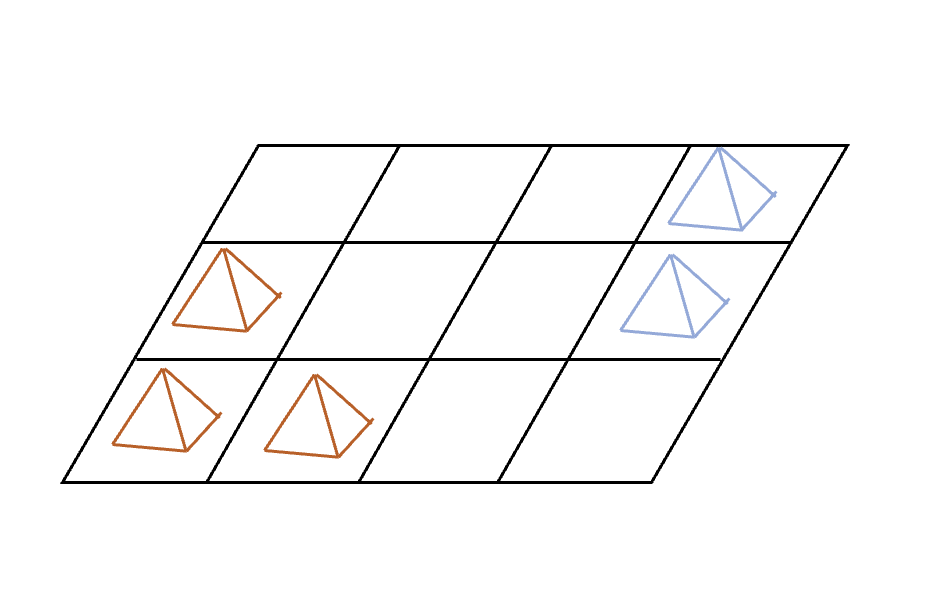
\includegraphics[scale=0.5]{tent.png} 
    \label{fig:my_label}
\end{figure}

\textbf{Input}: A nested array $A$ of $m \times n$ where 1 represents a tent and 0 represents an empty camping ground. 

[hint: You might want to locate all tents in one connected collection of tent first.] 

\Expecting{Pseudocode of the algorithm or a clear English description, \textbf{the algorithm should run in O(mn) time.}}


\pagebreak
\begin{Instruction}

\paragraph{Coding Problems} The following questions are to be submitted as a ".zip" file on Gradescope. 

\end{Instruction}

\section{Coding \Points{50}}
After completing the written portion of the assignment, you should submit it to \href{https://www.gradescope.com/courses/350304}{Gradescope}.

For the coding portion, get your starter \href{https://replit.com/team/COMP285/HW6-Code}{C++ code} or \href{https://replit.com/team/COMP285/HW6-Code-Python}{Python code}.

Note that the starter code also include a few test cases you can run on repl.it. However, the full test suite is the one run on Gradescope.

Please reference the \texttt{README.md} included in your starter code for detailed instructions.

\section*{Submitting the Assignment}

This assignment is a combination of written and programming questions. Both portions of the assignment should be submitted through \href{https://www.gradescope.com/courses/350304}{Gradescope}.

The "Homework 6: Fun with Graphs" assignment is the written portion, for which you should submit a \textbf{typed} response to the non-coding questions (questions 1-\ref{sec:last}). Each response should clearly be marked with its corresponding number. You are free to use the provided templates, print the questions and write your answers, or to simply type your responses on a blank document (whatever works for you).

The "Homework 6: Coding" is the programming portion of the assignment. For this portion, download the ".zip" file from replit and upload this ".zip" file as your answer to \href{https://www.gradescope.com/courses/350304}{Gradescope}. You can upload the assignment as many times as you want.


\end{document} 